\section{IRdet}

V~rámci této práce a ve spolupráci s~\textit{Laboratoří řízení kolejových
vozidel MENDELU} vznikla jednoduchá deska, která umožňuje připojení až 8 IR
čidel (viz \ref{ir}). Deska hlásí stav IR čidel pomocí opticky oddělených
8~digitálních výstupů. Výstupy desky lze připojit na vstupy \gls{mtbuni}
modulu, nebo například k~signalizačním diodám do pultu řízení obsluhy.
Deska \textit{IRdet} není nijak závislá na systému \gls{mtb}. V~této práci ji
však uvádíme, protože vznikla především proto, aby bylo možné plnohodnotně
nahradit současné \gls{mtbuni} moduly (s~přímou podporou IR čidel) použitím
nových modulů \gls{mtbuni} v4 a desek \textit{IRdet}.

\begin{table}[h]
	\begin{tabularx}{\textwidth}{lX}
		\toprule
		Vstupy & Až 8 IR čidel \\
		Výstupy & 8 digitálních opticky oddělených výstupů \\
		Napájení & 10–17 V~DC \\
		Proud IR diodami & nastavitelný osazením příslušného rezistoru \\
		\bottomrule
	\end{tabularx}
	\caption{Základní parametry desky \textit{IRdet}}
	\label{tab:mtbuni-params}
\end{table}

Schéma zapojení a deska plošných spojů jsou k~dispozici jako openhardware
projekt na \url{https://github.com/kmzbrnoI/irdet-ele}, firmware je psán jako
opensource projekt a je dispozici na
\url{https://github.com/kmzbrnoI/irdet-fw}.

Hlavní komponentou návrhu je procesor řady \textit{Atmega8*}. Lze osadit
libovolný z~procesorů \textit{ATmega8a}, \textit{ATmega88}, \textit{ATmega328}
a kompatibilní. Vstupy od fototranzistorů jsou zapojeny v~režimu kapacitní
vazby, viz \ref{cap-link}. Vysílací IR diody jsou buzeny přes tranzistory.
Proud do vysílacích diod je řízen omezovacím rezistorem na stabilizovaném
napětí.

Deska je tradičně navrhnuta především z~\textit{SMD} součástek (velikosti 0805)
jako dvoustranná s~cílem osazovat součástky automaticky. Napájení se očekává
ze stejného rozvodu jako je napájecí rozvod \gls{mtb} desek (ačkoliv to díky
optickému oddělení vstupů není nutné).

\begin{figure}[ht]
\subfigure{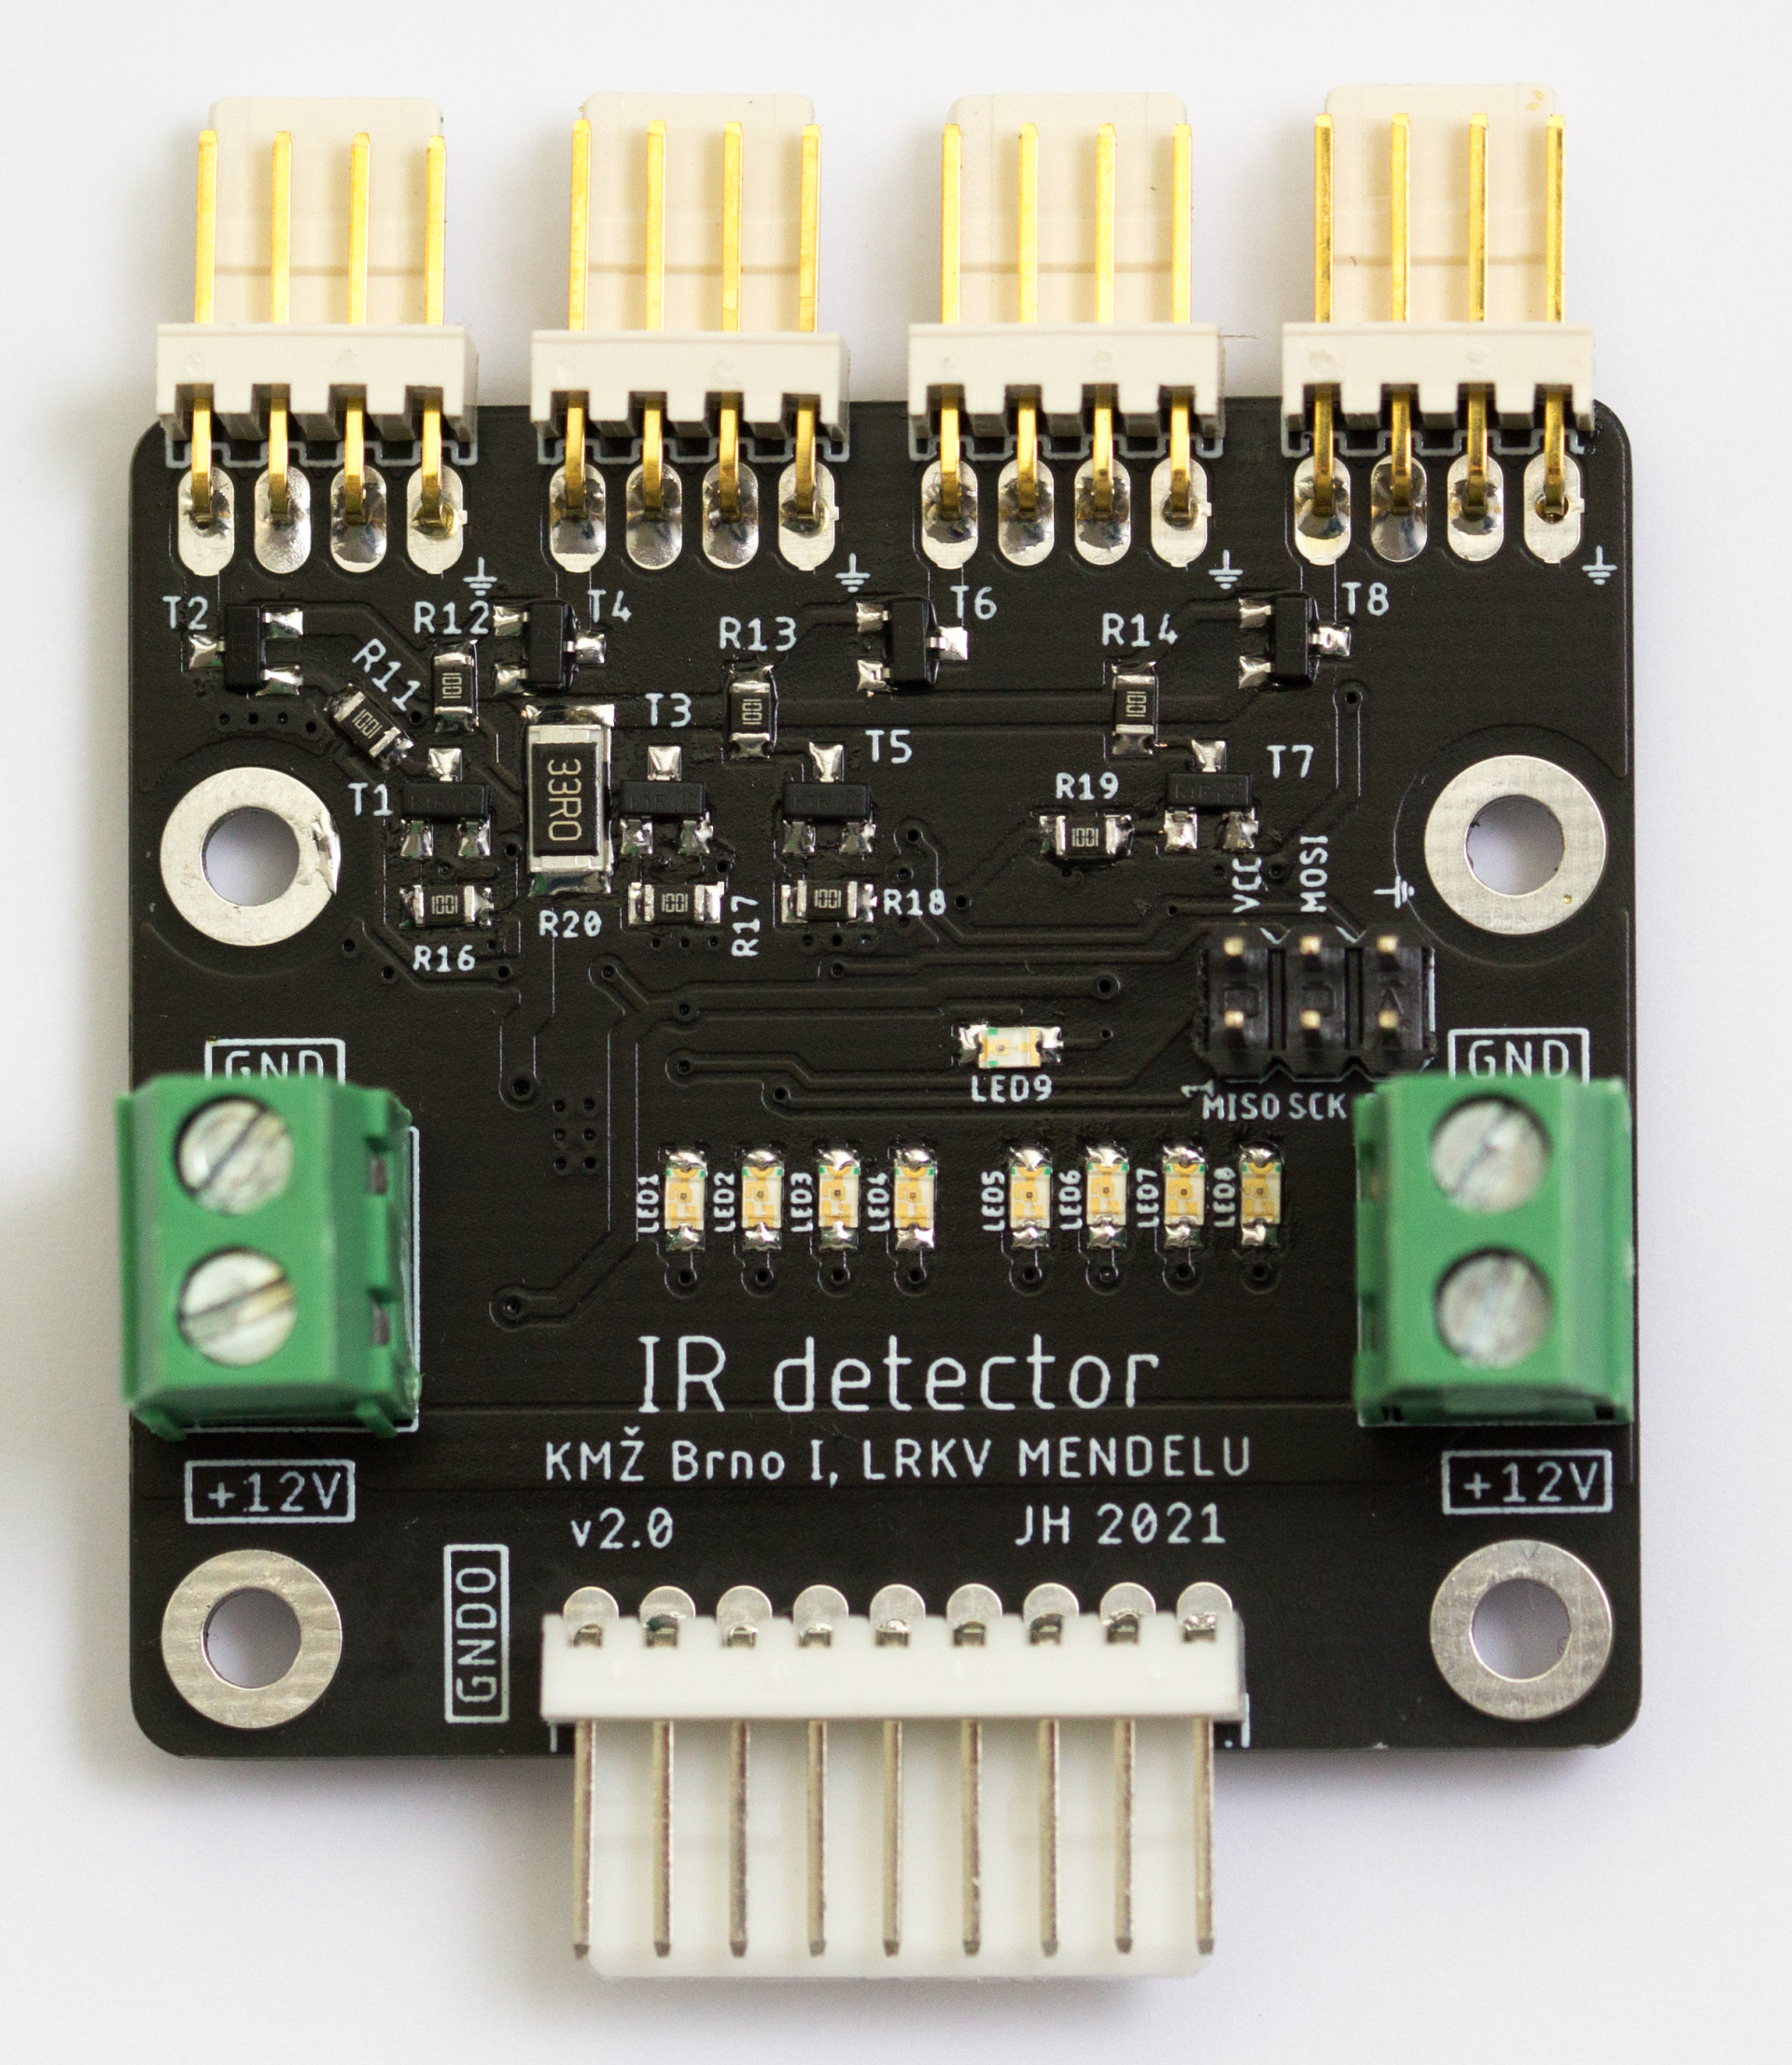
\includegraphics[width=0.5\textwidth]{data/irdet-front.jpg}}
\caption{Produkční verze desky IRdet}
\label{fig:irdet}
\end{figure}
